% Canimal CAN-USB: Datasheet and User Guide. Built by datasheet/build.sh; run from the repo root.
% Chapters come from the docs pages; every fact here must be on those pages or in the firmware manifest.
\documentclass[11pt,letterpaper]{report}

% Cover picture. Replace with a product photo when one exists.
\newcommand\CoverImage{public/assets/img/can-usb/can-usb-dimensions.jpg}
\newcommand\Brandmark{public/assets/img/brandmark.png}
\newcommand\DocTitle{Canimal CAN-USB}
\newcommand\DocSubtitle{Datasheet and User Guide}
\input{datasheet/build/version.tex}
\newcommand\VersionLine{Document version \DocCommit\ (\DocDate) \textperiodcentered\ Latest firmware \FirmwareLatest}

\usepackage[margin=0.9in,top=1in,bottom=1in,headheight=14pt]{geometry}
\usepackage{fontspec}
\setmainfont{SourceSans3}[Extension=.otf, UprightFont=*-Regular, BoldFont=*-Semibold,
  ItalicFont=*-RegularIt, BoldItalicFont=*-SemiboldIt]
\setmonofont{SourceCodePro}[Extension=.otf, UprightFont=*-Regular, BoldFont=*-Semibold,
  Scale=MatchLowercase]
\usepackage{microtype}
\usepackage[table]{xcolor}
\definecolor{brandyellow}{HTML}{FFC223}
\definecolor{brandgold}{HTML}{806112}
\definecolor{codebg}{HTML}{F5F5F2}
\definecolor{rulegray}{HTML}{BBBBBB}
\usepackage{graphicx,calc,array,longtable,booktabs,tabularx,enumitem,etoolbox}
\usepackage{fancyhdr,titlesec,caption,float}
\usepackage{fvextra}
\usepackage{tikz,pgfplots}
\usetikzlibrary{positioning,calc,shapes.misc}
\pgfplotsset{compat=1.18, every axis/.append style={font=\small},
  /pgf/number format/assume math mode=true}% numbers in the text font
\usepackage{xurl}
\usepackage[colorlinks,linkcolor=black,urlcolor=brandgold,
  pdftitle={Canimal CAN-USB: Datasheet and User Guide},pdfauthor={Canimal Systems Inc.},
  pdfcreator={},pdfproducer={}]{hyperref}

\urlstyle{same}
\setlength{\parindent}{0pt}
\setlength{\parskip}{0.55em}
\setlength{\emergencystretch}{3em}
\setlist{nosep,topsep=0.3em,leftmargin=1.4em}
% Macros pandoc's LaTeX output expects (from its default template).
\newcounter{none}% unnumbered tables
\makeatletter
\protected\def\pandocfootnotemark#1{\footnotemark{}%
  \expandafter\xdef\csname pandoc@fn@#1\endcsname{%
    \noexpand\pandoc@fnrestore
    {\unexpanded\expandafter{\@thefnmark}}%
    {\ifdefined\Hy@footnote@currentHref
       \unexpanded\expandafter{\Hy@footnote@currentHref}\fi}}}
\def\pandoc@fnrestore#1#2{%
  \gdef\@thefnmark{#1}%
  \ifdefined\Hy@footnote@currentHref\gdef\Hy@footnote@currentHref{#2}\fi}
\newcommand\pandocfootnotetext[1]{%
  \csname pandoc@fn@#1\endcsname\@footnotetext}
\makeatother
\providecommand{\tightlist}{\setlength{\itemsep}{0pt}\setlength{\parskip}{0pt}}
\captionsetup{font=small,labelfont=bf,justification=raggedright,singlelinecheck=false}
\renewcommand{\arraystretch}{1.25}

% Code from the docs pages: framed monospace, long lines wrap.
\DefineVerbatimEnvironment{codeblock}{Verbatim}{fontsize=\small,breaklines,breakanywhere,
  frame=leftline,framerule=2.5pt,rulecolor=\color{brandyellow},bgcolor=codebg,
  bgcolorpadding=4pt,xleftmargin=6pt}
\DefineVerbatimEnvironment{outputblock}{Verbatim}{fontsize=\small,breaklines,breakanywhere,
  frame=single,framerule=0.4pt,rulecolor=\color{rulegray},framesep=4pt,xleftmargin=4pt}

% Headings
\titleformat{\chapter}[block]{\normalfont\huge\bfseries}
  {\colorbox{brandyellow}{\makebox[1.2em]{\thechapter}}\hspace{0.5em}}{0pt}{}
\titlespacing*{\chapter}{0pt}{0pt}{1.4em}
\titleformat{\section}{\normalfont\Large\bfseries}{\thesection}{0.7em}{}
\titleformat{\subsection}{\normalfont\large\bfseries}{\thesubsection}{0.7em}{}
\titlespacing*{\section}{0pt}{1.4em}{0.4em}
\titlespacing*{\subsection}{0pt}{1.1em}{0.3em}
\setcounter{secnumdepth}{2}
\setcounter{tocdepth}{1}

% Header and footer on every page after the cover.
\pagestyle{fancy}
\renewcommand{\chaptermark}[1]{\markboth{\ifnum\value{chapter}>0\thechapter\quad\fi#1}{}}
\fancyhf{}
\fancyhead[L]{\small\bfseries\DocTitle: \DocSubtitle}
\fancyhead[R]{\small\leftmark}
\fancyfoot[L]{\footnotesize\VersionLine}
\fancyfoot[R]{\footnotesize Page \thepage}
\renewcommand{\headrule}{{\color{brandyellow}\hrule height 1.5pt}}
\renewcommand{\footrulewidth}{0.4pt}
\fancypagestyle{plain}{}

\begin{document}

% ---- Cover ----
\begin{titlepage}
\newgeometry{margin=0.9in}
\begin{tikzpicture}[remember picture,overlay]
  \fill[brandyellow] (current page.north west) rectangle ([yshift=-0.35in]current page.north east);
  \fill[black] (current page.south west) rectangle ([yshift=0.55in]current page.south east);
  \node[anchor=south,text=white,font=\small] at ([yshift=0.2in]current page.south)
    {docs.canimal.io \quad\textperiodcentered\quad canimal.io};
\end{tikzpicture}
\vspace*{0.1in}
\begin{minipage}[c]{0.75in}\includegraphics[width=\linewidth]{\Brandmark}\end{minipage}%
\hspace{0.15in}%
\begin{minipage}[c]{4in}\Large\bfseries Canimal Systems\end{minipage}

\vspace{0.7in}
{\fontsize{40}{46}\selectfont\bfseries \DocTitle\par}
\vspace{0.15in}
{\LARGE \DocSubtitle\par}
\vspace{0.1in}
{\large Three-channel CAN to USB adapter with CAN FD on CAN 0\par}

\vfill
\begin{center}
  \includegraphics[width=4.6in]{\CoverImage}
\end{center}
\vfill
{\color{brandyellow}\rule{\linewidth}{2pt}}\par
\VersionLine
\vspace{0.35in}
\restoregeometry
\end{titlepage}
\setcounter{page}{2}

% ---- Imprint ----
\thispagestyle{fancy}
\section*{Relevant products}
\begin{tabularx}{\linewidth}{@{}lX@{}}
\toprule
\textbf{Product} & \textbf{Description} \\
\midrule
Canimal CAN-USB & Three-channel CAN to USB adapter: classic CAN on CAN 0, CAN 1 and CAN 2;
CAN FD on CAN 0. Product page: \url{https://canimal.io/products} \\
\bottomrule
\end{tabularx}

\vspace{1.5em}
\section*{Imprint}
Canimal Systems Inc.\\
\url{https://canimal.io}\\
Documentation: \url{https://docs.canimal.io}

Specifications may change without notice. The online documentation at
\url{https://docs.canimal.io} is current; this document is generated from it.

This edition: \VersionLine.

\textcopyright\ \DocYear\ Canimal Systems Inc. All rights reserved.

\clearpage
\tableofcontents
\markboth{Contents}{}% header without the class's capitals

% ---- Chapters ----
\chapter{Introduction}
\input{datasheet/build/guide-intro.tex}

\section{Block diagram}
\begin{figure}[H]
  \centering
  % CAN-USB block diagram. Facts: specs page (USB, channels, CAN FD on CAN 0, termination) and the
% front-panel picture on it (TX, RX and TERM indicators per channel).
\begin{tikzpicture}[
    font=\small, >=stealth, line width=0.6pt,
    blk/.style={draw, rounded corners=2pt, align=center, fill=white},
    term/.style={draw, rounded corners=2pt, align=center, font=\footnotesize, fill=codebg},
    conn/.style={draw, align=center, fill=brandyellow, minimum width=1.9cm, minimum height=0.95cm},
    bus/.style={line width=1.4pt},
  ]
  % USB side
  \node[blk, minimum height=1.6cm, text width=2.5cm] (usb) at (0,-1.9)
    {\textbf{USB-C} to host\\USB 2.0 High Speed\\480 Mbit/s\\data and power};
  \node[blk, minimum height=5.3cm, text width=1.9cm] (ctrl) at (3.3,-1.9) {\textbf{Controller}\\[2pt]3 CAN\\channels};
  \draw[<->, bus] (usb) -- (ctrl);
  \node[font=\footnotesize, align=center, below=0.15cm of usb] {powered from USB};

  \foreach \ch/\y/\fd in {0/0/{CAN FD}, 1/-1.9/{classic CAN}, 2/-3.8/{classic CAN}} {
    \node[blk, text width=2.3cm, minimum height=0.95cm] (tr\ch) at (7.0,\y)
      {Transceiver\\[-1pt]{\footnotesize ISO 11898-2}};
    \draw[<->, bus] (ctrl.east |- tr\ch) -- node[above, font=\scriptsize] {\fd} (tr\ch);
    \node[conn] (ds\ch) at (13.0,\y) {\textbf{CAN \ch}\\[-1pt]{\footnotesize D-Sub 9}};
    \draw[bus] (tr\ch) -- (ds\ch);
    \node[term, text width=2.6cm] (rt\ch) at (10.0,\y-0.8)
      {120\,Ω terminator,\\[-1pt]software switched};
    \node[draw, circle, fill=brandyellow, inner sep=1.6pt, label={[font=\scriptsize]right:TERM}]
      at ([xshift=0.25cm]rt\ch.east) {};
    \draw (rt\ch.north) -- (rt\ch.north |- tr\ch);
    \fill (rt\ch.north |- tr\ch) circle (1.7pt);
  }
  \draw[dashed, rounded corners=4pt, rulegray]
    ([xshift=-0.25cm, yshift=0.55cm]usb.west |- tr0.north) rectangle
    ([xshift=0.25cm, yshift=-0.95cm]ds2.east |- rt2.south);
  \node[anchor=south east, font=\footnotesize\bfseries, text=brandgold]
    at ([xshift=0.25cm, yshift=0.55cm]ds0.east |- tr0.north) {Canimal CAN-USB};
\end{tikzpicture}

  \caption{CAN-USB block diagram. Termination is switched by software for each channel, with a
    TERM indicator next to the channel's TX and RX indicators.}
\end{figure}

\chapter{Connectors and channels}
\input{datasheet/build/guide-connectors.tex}
\begin{figure}[H]
  \centering
  % 9-pin D-Sub, male, pin side. Pin signals from the user guide's CiA 106 table; other pins unlabelled.
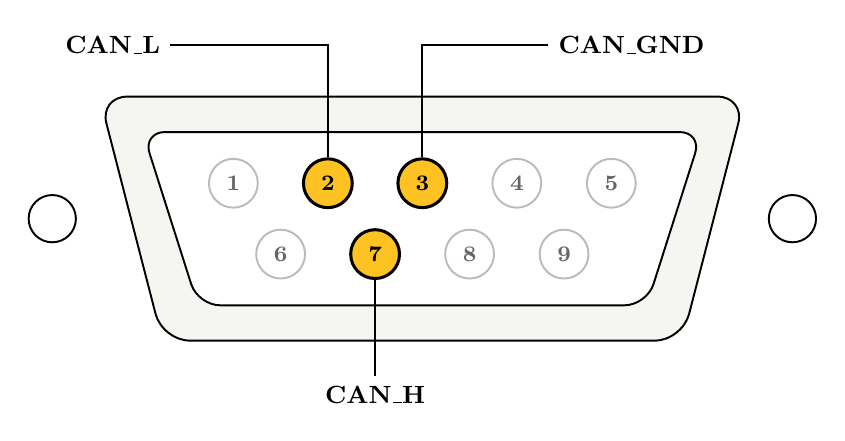
\begin{tikzpicture}[
    font=\small, line width=0.7pt,
    pin/.style={circle, draw, minimum size=0.62cm, inner sep=0pt, font=\footnotesize\bfseries},
    can/.style={pin, fill=brandyellow, line width=1.1pt},
    other/.style={pin, fill=white, draw=rulegray, text=black!60},
    lbl/.style={font=\small\bfseries},
  ]
  % Shell and inner face (trapezoid, wider at the top)
  \draw[rounded corners=10pt, fill=codebg] (-4.1,1.55) -- (4.1,1.55) -- (3.3,-1.55) -- (-3.3,-1.55) -- cycle;
  \draw[rounded corners=8pt, fill=white] (-3.55,1.1) -- (3.55,1.1) -- (2.85,-1.1) -- (-2.85,-1.1) -- cycle;
  \foreach \x in {-4.7,4.7} \draw[fill=white] (\x,0) circle (0.3);

  % Pins 1-5 on top, 6-9 below, left to right
  \foreach \n/\x in {1/-2.4,4/1.2,5/2.4} \node[other] (p\n) at (\x,0.45) {\n};
  \foreach \n/\x in {6/-1.8,8/0.6,9/1.8} \node[other] (p\n) at (\x,-0.45) {\n};
  \node[can] (p2) at (-1.2,0.45) {2};
  \node[can] (p3) at (0,0.45) {3};
  \node[can] (p7) at (-0.6,-0.45) {7};

  \draw (p2) |- (-3.2,2.2) node[lbl, left] {CAN\_L};
  \draw (p3) |- (1.6,2.2) node[lbl, right] {CAN\_GND};
  \draw (p7) -- ++(0,-1.55) node[lbl, below] {CAN\_H};
\end{tikzpicture}

  \caption{9-pin D-Sub connector (male, pin side) with the CiA 106 CAN pins. Each of CAN 0,
    CAN 1 and CAN 2 has one.}
\end{figure}

\chapter{User guide}
\input{datasheet/build/guide-linux.tex}

\chapter{Technical specifications}
\input{datasheet/build/specs.tex}

\section{Bus limit}
% Theoretical maximum frames per second a CAN bus can carry. Computed here, not measured.
% Worst-case bit stuffing: floor((n-1)/4) stuff bits over the n bits from SOF to the end of the data
% field. Trailer: CRC delimiter 1, ACK 2, EOF 7, interframe space 3 = 13 bits.
\pgfmathtruncatemacro\stdstuffed{34 + 8*8}% SOF, 11-bit ID, RTR, IDE, r0, DLC, 8 data bytes, CRC-15
\pgfmathtruncatemacro\stdbits{\stdstuffed + floor((\stdstuffed - 1)/4) + 13}
\pgfmathtruncatemacro\extstuffed{54 + 8*8}% the same with a 29-bit ID (SRR, IDE, r1, r0)
\pgfmathtruncatemacro\extbits{\extstuffed + floor((\extstuffed - 1)/4) + 13}
% CAN FD, 11-bit ID, BRS on, 64 data bytes. Arbitration phase: SOF to BRS (17 bits) and the trailer.
% Data phase: ESI, DLC and data (517 bits), their stuff bits, and the CRC field (stuff count 4,
% CRC-21, 7 fixed stuff bits = 32 bits).
\pgfmathtruncatemacro\fdarbstuff{floor((17 - 1)/4)}
\pgfmathtruncatemacro\fdnombits{17 + \fdarbstuff + 13}
\pgfmathtruncatemacro\fddatabits{517 + floor((17 + 517 - 1)/4) - \fdarbstuff + 32}
\edef\stdmax{\directlua{tex.sprint(math.floor(1e6 / \stdbits))}}% pgfmath stops at 16383
\edef\extmax{\directlua{tex.sprint(math.floor(1e6 / \extbits))}}
\begin{figure}[H]
  \centering
  \begin{tikzpicture}
    \begin{axis}[
        xmode=log, ymode=log, width=0.9\linewidth, height=8.2cm,
        xmin=1e4, xmax=1e7, ymin=50, ymax=2e4,
        xtick={1e4,1e5,1e6,1e7}, xticklabels={10 k,100 k,1 M,10 M},
        ytick={100,1000,10000}, yticklabels={100,1\,000,10\,000},
        xlabel={Bit rate (bit/s); for CAN FD, the data-phase bit rate},
        ylabel={Frames per second},
        grid=both, grid style={rulegray!50}, major grid style={rulegray},
        legend pos=south east, legend cell align=left, legend style={font=\small},
        tick label style={font=\small},
      ]
      \addplot[domain=1e4:1e6, samples=2, very thick, black] {x/\stdbits};
      \addlegendentry{Classic CAN, standard ID, 8 bytes}
      \addplot[domain=1e4:1e6, samples=2, very thick, black, dashed] {x/\extbits};
      \addlegendentry{Classic CAN, extended ID, 8 bytes}
      \addplot[very thick, brandgold, mark=*, mark options={fill=brandyellow, draw=black},
          nodes near coords={\pgfmathprintnumber[fixed, precision=0, 1000 sep={\,}]{\pgfplotspointmeta}},
          nodes near coords style={font=\footnotesize, text=black, anchor=north},
          point meta=rawy]
        table[x=dbitrate, y expr={1/(\fdnombits/500000 + \fddatabits/\thisrow{dbitrate})}]
        {datasheet/data/fd-data-rates.csv};
      \addlegendentry{CAN FD, standard ID, 64 bytes, 500 kbit/s arbitration}
    \end{axis}
  \end{tikzpicture}
  \caption{Bus limit (theoretical), not a measurement of the CAN-USB.}
\end{figure}

{\small
\textbf{How this is computed.} Frames per second = bit rate ÷ bits per frame, with worst-case bit
stuffing (one stuff bit for every 4 bits after the first, over the bits from start of frame to the
end of the data field) and a 3-bit interframe space. Classic CAN with 8 data bytes: \stdbits\ bits
with a standard ID and \extbits\ bits with an extended ID, so at most \stdmax\ and \extmax\ frames
per second at 1 Mbit/s. CAN FD with 64 data bytes and bit-rate switching: \fdnombits\ bits at the
arbitration bit rate and \fddatabits\ bits at the data bit rate (including the CRC-21 field with its
fixed stuff bits); the bit-rate switch and CRC delimiter bits are counted at the arbitration rate.
\par}


% ---- Appendices ----
\appendix
\chapter{Dimension drawing}
\begin{figure}[H]
  \centering
  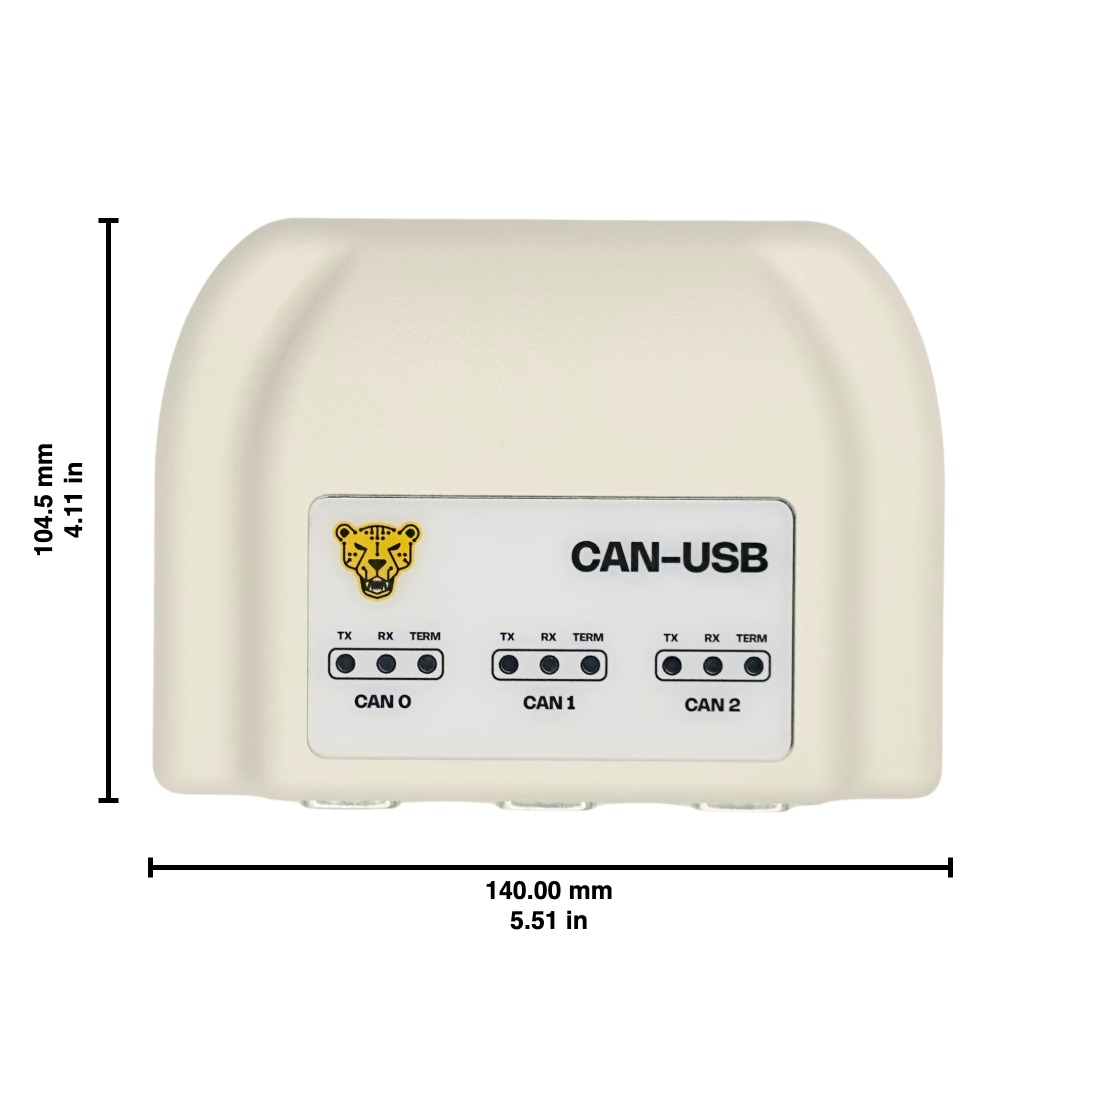
\includegraphics[width=0.85\linewidth]{public/assets/img/can-usb/can-usb-dimensions.jpg}
  \caption{CAN-USB, top view. Width 140.00 mm (5.51 in), length 104.50 mm (4.11 in),
    height 36.50 mm (1.44 in).}
\end{figure}

\end{document}
